%-*-latex-*-
\tinysidebar{\debug{exercises/3n3-5-42-n5-n2-1/main.tex}}
The following are plots of $|f(n)|$ and $g(n) = n^4$:
%-*-latex-*-

\begin{center}
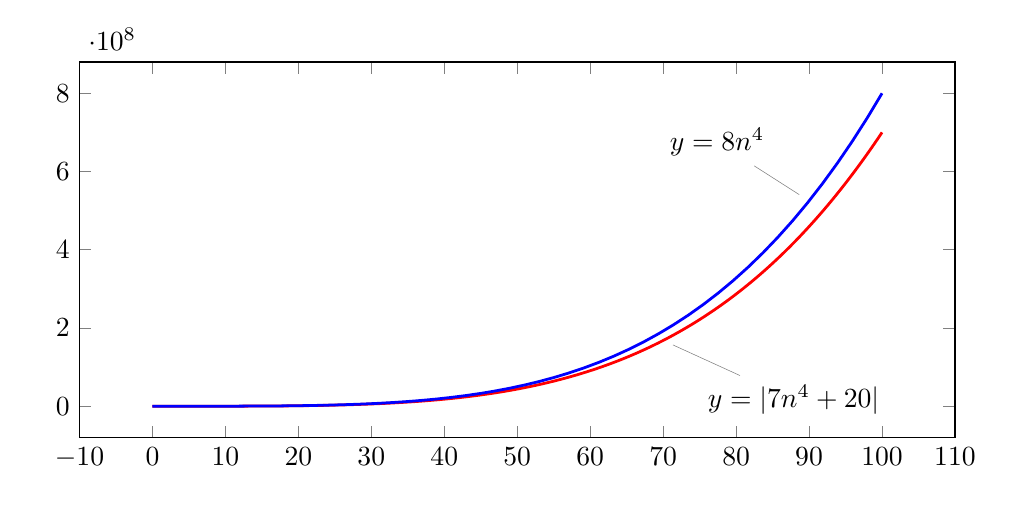
\begin{tikzpicture}[line width=1]
\begin{axis}[width=5in, height=2.5in,
             scatter/classes={a={mark=*,draw=black}},
             xlabel={\mbox{}},
             xlabel style={name=xlabel}, 
             ylabel={\mbox{}}, 
             legend style={
                at={(xlabel.south)},
                yshift=-1ex,
                anchor=north,
                legend cell align=left,
                },
        ]
]
\addplot[draw=red, line width=1] coordinates {(0.0,20.0)
(0.1001,20.0007)
(0.2002,20.0112)
(0.3003,20.0569)
(0.4004,20.1799)
(0.5005,20.4393)
(0.6006,20.9108)
(0.7007,21.6874)
(0.8008,22.8787)
(0.9009,24.6111)
(1.001,27.0281)
(1.1011,30.2898)
(1.2012,34.5734)
(1.3013,40.0729)
(1.4014,46.999)
(1.5015,55.5796)
(1.6016,66.0592)
(1.7017,78.6991)
(1.8018,93.7779)
(1.9019,111.5905)
(2.002,132.4491)
(2.1021,156.6826)
(2.2022,184.6368)
(2.3023,216.6742)
(2.4024,253.1745)
(2.5025,294.534)
(2.6026,341.1659)
(2.7027,393.5005)
(2.8028,451.9845)
(2.9029,517.082)
(3.003,589.2737)
(3.1031,669.057)
(3.2032,756.9466)
(3.3033,853.4736)
(3.4034,959.1863)
(3.5035,1074.6498)
(3.6036,1200.4459)
(3.7037,1337.1735)
(3.8038,1485.4482)
(3.9039,1645.9026)
(4.004,1819.186)
(4.1041,2005.9647)
(4.2042,2206.9218)
(4.3043,2422.7573)
(4.4044,2654.1882)
(4.5045,2901.948)
(4.6046,3166.7875)
(4.7047,3449.474)
(4.8048,3750.792)
(4.9049,4071.5426)
(5.005,4412.5438)
(5.1051,4774.6307)
(5.2052,5158.655)
(5.3053,5565.4854)
(5.4054,5996.0074)
(5.5055,6451.1234)
(5.6056,6931.7528)
(5.7057,7438.8315)
(5.8058,7973.3128)
(5.9059,8536.1663)
(6.006,9128.3789)
(6.1061,9750.9542)
(6.2062,10404.9126)
(6.3063,11091.2915)
(6.4064,11811.1451)
(6.5065,12565.5445)
(6.6066,13355.5776)
(6.7067,14182.3492)
(6.8068,15046.981)
(6.9069,15950.6116)
(7.007,16894.3964)
(7.1071,17879.5076)
(7.2072,18907.1345)
(7.3073,19978.483)
(7.4074,21094.7759)
(7.5075,22257.2532)
(7.6076,23467.1713)
(7.7077,24725.8038)
(7.8078,26034.441)
(7.9079,27394.3901)
(8.008,28806.9753)
(8.1081,30273.5374)
(8.2082,31795.4344)
(8.3083,33374.0409)
(8.4084,35010.7484)
(8.5085,36706.9654)
(8.6086,38464.1172)
(8.7087,40283.6459)
(8.8088,42167.0105)
(8.9089,44115.6871)
(9.009,46131.1682)
(9.1091,48214.9636)
(9.2092,50368.5997)
(9.3093,52593.6199)
(9.4094,54891.5845)
(9.5095,57264.0705)
(9.6096,59712.672)
(9.7097,62238.9996)
(9.8098,64844.6812)
(9.9099,67531.3613)
(10.01,70300.7014)
(10.1101,73154.3797)
(10.2102,76094.0914)
(10.3103,79121.5486)
(10.4104,82238.4801)
(10.5105,85446.6318)
(10.6106,88747.7663)
(10.7107,92143.663)
(10.8108,95636.1184)
(10.9109,99226.9456)
(11.011,102917.9749)
(11.1111,106711.0532)
(11.2112,110608.0443)
(11.3113,114610.8289)
(11.4114,118721.3047)
(11.5115,122941.386)
(11.6116,127273.0042)
(11.7117,131718.1075)
(11.8118,136278.6608)
(11.9119,140956.6462)
(12.012,145754.0624)
(12.1121,150672.9251)
(12.2122,155715.2667)
(12.3123,160883.1367)
(12.4124,166178.6013)
(12.5125,171603.7437)
(12.6126,177160.6637)
(12.7127,182851.4784)
(12.8128,188678.3213)
(12.9129,194643.3431)
(13.013,200748.7113)
(13.1131,206996.6101)
(13.2132,213389.2408)
(13.3133,219928.8214)
(13.4134,226617.5869)
(13.5135,233457.789)
(13.6136,240451.6964)
(13.7137,247601.5946)
(13.8138,254909.786)
(13.9139,262378.59)
(14.014,270010.3425)
(14.1141,277807.3967)
(14.2142,285772.1223)
(14.3143,293906.9062)
(14.4144,302214.1519)
(14.5145,310696.2798)
(14.6146,319355.7274)
(14.7147,328194.9488)
(14.8148,337216.415)
(14.9149,346422.6141)
(15.015,355816.0508)
(15.1151,365399.2469)
(15.2152,375174.7407)
(15.3153,385145.0878)
(15.4154,395312.8605)
(15.5155,405680.6477)
(15.6156,416251.0557)
(15.7157,427026.7072)
(15.8158,438010.242)
(15.9159,449204.3167)
(16.016,460611.6047)
(16.1161,472234.7965)
(16.2162,484076.5992)
(16.3163,496139.7369)
(16.4164,508426.9506)
(16.5165,520940.998)
(16.6166,533684.654)
(16.7167,546660.7099)
(16.8168,559871.9742)
(16.9169,573321.2723)
(17.017,587011.4462)
(17.1171,600945.355)
(17.2172,615125.8745)
(17.3173,629555.8976)
(17.4174,644238.3338)
(17.5175,659176.1096)
(17.6176,674372.1685)
(17.7177,689829.4705)
(17.8178,705550.9928)
(17.9179,721539.7294)
(18.018,737798.691)
(18.1181,754330.9055)
(18.2182,771139.4172)
(18.3183,788227.2878)
(18.4184,805597.5953)
(18.5185,823253.4351)
(18.6186,841197.9192)
(18.7187,859434.1764)
(18.8188,877965.3524)
(18.9189,896794.6101)
(19.019,915925.1287)
(19.1191,935360.1048)
(19.2192,955102.7515)
(19.3193,975156.299)
(19.4194,995523.9941)
(19.5195,1016209.1008)
(19.6196,1037214.8998)
(19.7197,1058544.6885)
(19.8198,1080201.7816)
(19.9199,1102189.5101)
(20.02,1124511.2224)
(20.1201,1147170.2835)
(20.2202,1170170.0753)
(20.3203,1193513.9965)
(20.4204,1217205.4628)
(20.5205,1241247.9067)
(20.6206,1265644.7776)
(20.7207,1290399.5417)
(20.8208,1315515.6822)
(20.9209,1340996.699)
(21.021,1366846.1089)
(21.1211,1393067.4458)
(21.2212,1419664.2601)
(21.3213,1446640.1192)
(21.4214,1473998.6077)
(21.5215,1501743.3265)
(21.6216,1529877.8937)
(21.7217,1558405.9444)
(21.8218,1587331.1302)
(21.9219,1616657.1198)
(22.022,1646387.5988)
(22.1221,1676526.2694)
(22.2222,1707076.8511)
(22.3223,1738043.0798)
(22.4224,1769428.7087)
(22.5225,1801237.5074)
(22.6226,1833473.2629)
(22.7227,1866139.7786)
(22.8228,1899240.875)
(22.9229,1932780.3894)
(23.023,1966762.1761)
(23.1231,2001190.1061)
(23.2232,2036068.0673)
(23.3233,2071399.9646)
(23.4234,2107189.7195)
(23.5235,2143441.2706)
(23.6236,2180158.5734)
(23.7237,2217345.6)
(23.8238,2255006.3397)
(23.9239,2293144.7983)
(24.024,2331764.9989)
(24.1241,2370870.981)
(24.2242,2410466.8014)
(24.3243,2450556.5334)
(24.4244,2491144.2675)
(24.5245,2532234.1108)
(24.6246,2573830.1874)
(24.7247,2615936.6382)
(24.8248,2658557.6211)
(24.9249,2701697.3107)
(25.025,2745359.8985)
(25.1251,2789549.593)
(25.2252,2834270.6195)
(25.3253,2879527.2201)
(25.4254,2925323.6537)
(25.5255,2971664.1963)
(25.6256,3018553.1406)
(25.7257,3065994.7963)
(25.8258,3113993.4898)
(25.9259,3162553.5644)
(26.026,3211679.3804)
(26.1261,3261375.3149)
(26.2262,3311645.7617)
(26.3263,3362495.1318)
(26.4264,3413927.8528)
(26.5265,3465948.3693)
(26.6266,3518561.1426)
(26.7267,3571770.6511)
(26.8268,3625581.3899)
(26.9269,3679997.871)
(27.027,3735024.6234)
(27.1271,3790666.1928)
(27.2272,3846927.1417)
(27.3273,3903812.0498)
(27.4274,3961325.5133)
(27.5275,4019472.1454)
(27.6276,4078256.5764)
(27.7277,4137683.4531)
(27.8278,4197757.4393)
(27.9279,4258483.2158)
(28.028,4319865.4801)
(28.1281,4381908.9467)
(28.2282,4444618.3468)
(28.3283,4507998.4286)
(28.4284,4572053.9571)
(28.5285,4636789.7143)
(28.6286,4702210.4989)
(28.7287,4768321.1265)
(28.8288,4835126.4296)
(28.9289,4902631.2577)
(29.029,4970840.4769)
(29.1291,5039758.9703)
(29.2292,5109391.638)
(29.3293,5179743.3967)
(29.4294,5250819.1801)
(29.5295,5322623.9389)
(29.6296,5395162.6405)
(29.7297,5468440.2691)
(29.8298,5542461.826)
(29.9299,5617232.3292)
(30.03,5692756.8136)
(30.1301,5769040.331)
(30.2302,5846087.95)
(30.3303,5923904.7561)
(30.4304,6002495.8518)
(30.5305,6081866.3562)
(30.6306,6162021.4055)
(30.7307,6242966.1526)
(30.8308,6324705.7674)
(30.9309,6407245.4367)
(31.031,6490590.364)
(31.1311,6574745.7697)
(31.2312,6659716.8912)
(31.3313,6745508.9827)
(31.4314,6832127.3151)
(31.5315,6919577.1765)
(31.6316,7007863.8716)
(31.7317,7096992.7221)
(31.8318,7186969.0665)
(31.9319,7277798.2602)
(32.032,7369485.6754)
(32.1321,7462036.7012)
(32.2322,7555456.7438)
(32.3323,7649751.2258)
(32.4324,7744925.5871)
(32.5325,7840985.2842)
(32.6326,7937935.7906)
(32.7327,8035782.5966)
(32.8328,8134531.2095)
(32.9329,8234187.1532)
(33.033,8334755.9688)
(33.1331,8436243.214)
(33.2332,8538654.4634)
(33.3333,8641995.3086)
(33.4334,8746271.3581)
(33.5335,8851488.237)
(33.6336,8957651.5876)
(33.7337,9064767.0687)
(33.8338,9172840.3564)
(33.9339,9281877.1432)
(34.034,9391883.1389)
(34.1341,9502864.0699)
(34.2342,9614825.6795)
(34.3343,9727773.728)
(34.4344,9841713.9924)
(34.5345,9956652.2666)
(34.6346,10072594.3615)
(34.7347,10189546.1047)
(34.8348,10307513.3408)
(34.9349,10426501.9312)
(35.035,10546517.7542)
(35.1351,10667566.7049)
(35.2352,10789654.6953)
(35.3353,10912787.6544)
(35.4354,11036971.5277)
(35.5355,11162212.2781)
(35.6356,11288515.8849)
(35.7357,11415888.3445)
(35.8358,11544335.6702)
(35.9359,11673863.8919)
(36.036,11804479.0567)
(36.1361,11936187.2283)
(36.2362,12068994.4876)
(36.3363,12202906.9319)
(36.4364,12337930.6758)
(36.5365,12474071.8505)
(36.6366,12611336.6041)
(36.7367,12749731.1018)
(36.8368,12889261.5254)
(36.9369,13029934.0736)
(37.037,13171754.9621)
(37.1371,13314730.4234)
(37.2372,13458866.7068)
(37.3373,13604170.0785)
(37.4374,13750646.8217)
(37.5375,13898303.2363)
(37.6376,14047145.6392)
(37.7377,14197180.364)
(37.8378,14348413.7613)
(37.9379,14500852.1985)
(38.038,14654502.06)
(38.1381,14809369.7468)
(38.2382,14965461.6771)
(38.3383,15122784.2857)
(38.4384,15281344.0245)
(38.5385,15441147.3619)
(38.6386,15602200.7836)
(38.7387,15764510.792)
(38.8388,15928083.9061)
(38.9389,16092926.6623)
(39.039,16259045.6133)
(39.1391,16426447.3291)
(39.2392,16595138.3964)
(39.3393,16765125.4188)
(39.4394,16936415.0166)
(39.5395,17109013.8273)
(39.6396,17282928.5049)
(39.7397,17458165.7205)
(39.8398,17634732.1621)
(39.9399,17812634.5344)
(40.04,17991879.559)
(40.1401,18172473.9745)
(40.2402,18354424.5363)
(40.3403,18537738.0166)
(40.4404,18722421.2045)
(40.5405,18908480.906)
(40.6406,19095923.9439)
(40.7407,19284757.158)
(40.8408,19474987.4049)
(40.9409,19666621.558)
(41.041,19859666.5076)
(41.1411,20054129.1609)
(41.2412,20250016.442)
(41.3413,20447335.2917)
(41.4414,20646092.668)
(41.5415,20846295.5454)
(41.6416,21047950.9154)
(41.7417,21251065.7866)
(41.8418,21455647.184)
(41.9419,21661702.1498)
(42.042,21869237.7431)
(42.1421,22078261.0397)
(42.2422,22288779.1323)
(42.3423,22500799.1305)
(42.4424,22714328.1608)
(42.5425,22929373.3665)
(42.6426,23145941.9079)
(42.7427,23364040.9619)
(42.8428,23583677.7225)
(42.9429,23804859.4005)
(43.043,24027593.2235)
(43.1431,24251886.4362)
(43.2432,24477746.2999)
(43.3433,24705180.0929)
(43.4434,24934195.1103)
(43.5435,25164798.6641)
(43.6436,25396998.0832)
(43.7437,25630800.7134)
(43.8438,25866213.9171)
(43.9439,26103245.074)
(44.044,26341901.5804)
(44.1441,26582190.8494)
(44.2442,26824120.3111)
(44.3443,27067697.4125)
(44.4444,27312929.6174)
(44.5445,27559824.4065)
(44.6446,27808389.2773)
(44.7447,28058631.7442)
(44.8448,28310559.3385)
(44.9449,28564179.6084)
(45.045,28819500.1188)
(45.1451,29076528.4517)
(45.2452,29335272.2058)
(45.3453,29595738.9967)
(45.4454,29857936.4569)
(45.5455,30121872.2358)
(45.6456,30387553.9995)
(45.7457,30654989.4312)
(45.8458,30924186.2308)
(45.9459,31195152.1151)
(46.046,31467894.8179)
(46.1461,31742422.0896)
(46.2462,32018741.6977)
(46.3463,32296861.4265)
(46.4464,32576789.0772)
(46.5465,32858532.4677)
(46.6466,33142099.433)
(46.7467,33427497.8248)
(46.8468,33714735.5118)
(46.9469,34003820.3794)
(47.047,34294760.33)
(47.1471,34587563.2829)
(47.2472,34882237.1741)
(47.3473,35178789.9566)
(47.4474,35477229.6002)
(47.5475,35777564.0917)
(47.6476,36079801.4345)
(47.7477,36383949.6492)
(47.8478,36690016.773)
(47.9479,36998010.8602)
(48.048,37307939.9816)
(48.1481,37619812.2253)
(48.2482,37933635.696)
(48.3483,38249418.5153)
(48.4484,38567168.8218)
(48.5485,38886894.7708)
(48.6486,39208604.5346)
(48.7487,39532306.3023)
(48.8488,39858008.2798)
(48.9489,40185718.69)
(49.049,40515445.7726)
(49.1491,40847197.7841)
(49.2492,41180982.9981)
(49.3493,41516809.7048)
(49.4494,41854686.2114)
(49.5495,42194620.842)
(49.6496,42536621.9374)
(49.7497,42880697.8555)
(49.8498,43226856.9709)
(49.9499,43575107.6751)
(50.0501,43925458.3765)
(50.1502,44277917.5004)
(50.2503,44632493.4888)
(50.3504,44989194.8008)
(50.4505,45348029.9121)
(50.5506,45709007.3156)
(50.6507,46072135.5208)
(50.7508,46437423.0542)
(50.8509,46804878.4591)
(50.951,47174510.2956)
(51.0511,47546327.1409)
(51.1512,47920337.5888)
(51.2513,48296550.2502)
(51.3514,48674973.7526)
(51.4515,49055616.7408)
(51.5516,49438487.8759)
(51.6517,49823595.8363)
(51.7518,50210949.3172)
(51.8519,50600557.0305)
(51.952,50992427.705)
(52.0521,51386570.0865)
(52.1522,51782992.9377)
(52.2523,52181705.0379)
(52.3524,52582715.1835)
(52.4525,52986032.1878)
(52.5526,53391664.8807)
(52.6527,53799622.1092)
(52.7528,54209912.7371)
(52.8529,54622545.6451)
(52.953,55037529.7307)
(53.0531,55454873.9083)
(53.1532,55874587.1092)
(53.2533,56296678.2815)
(53.3534,56721156.3903)
(53.4535,57148030.4173)
(53.5536,57577309.3615)
(53.6537,58009002.2382)
(53.7538,58443118.0801)
(53.8539,58879665.9365)
(53.954,59318654.8736)
(54.0541,59760093.9744)
(54.1542,60203992.339)
(54.2543,60650359.084)
(54.3544,61099203.3433)
(54.4545,61550534.2673)
(54.5546,62004361.0235)
(54.6547,62460692.7961)
(54.7548,62919538.7863)
(54.8549,63380908.2122)
(54.955,63844810.3085)
(55.0551,64311254.3271)
(55.1552,64780249.5365)
(55.2553,65251805.2223)
(55.3554,65725930.6868)
(55.4555,66202635.2492)
(55.5556,66681928.2457)
(55.6557,67163819.0291)
(55.7558,67648316.9693)
(55.8559,68135431.453)
(55.956,68625171.8838)
(56.0561,69117547.682)
(56.1562,69612568.2849)
(56.2563,70110243.1468)
(56.3564,70610581.7387)
(56.4565,71113593.5483)
(56.5566,71619288.0806)
(56.6567,72127674.8571)
(56.7568,72638763.4164)
(56.8569,73152563.3137)
(56.957,73669084.1214)
(57.0571,74188335.4285)
(57.1572,74710326.841)
(57.2573,75235067.9817)
(57.3574,75762568.4903)
(57.4575,76292838.0235)
(57.5576,76825886.2545)
(57.6577,77361722.8738)
(57.7578,77900357.5886)
(57.8579,78441800.1227)
(57.958,78986060.2172)
(58.0581,79533147.6298)
(58.1582,80083072.1352)
(58.2583,80635843.5248)
(58.3584,81191471.6071)
(58.4585,81749966.2073)
(58.5586,82311337.1674)
(58.6587,82875594.3466)
(58.7588,83442747.6205)
(58.8589,84012806.882)
(58.959,84585782.0405)
(59.0591,85161683.0227)
(59.1592,85740519.7717)
(59.2593,86322302.2477)
(59.3594,86907040.4278)
(59.4595,87494744.306)
(59.5596,88085423.8929)
(59.6597,88679089.2163)
(59.7598,89275750.3206)
(59.8599,89875417.2673)
(59.96,90478100.1346)
(60.0601,91083809.0176)
(60.1602,91692554.0283)
(60.2603,92304345.2956)
(60.3604,92919192.9651)
(60.4605,93537107.1995)
(60.5606,94158098.1783)
(60.6607,94782176.0977)
(60.7608,95409351.1709)
(60.8609,96039633.6281)
(60.961,96673033.7161)
(61.0611,97309561.6987)
(61.1612,97949227.8566)
(61.2613,98592042.4873)
(61.3614,99238015.9052)
(61.4615,99887158.4416)
(61.5616,100539480.4446)
(61.6617,101194992.2792)
(61.7618,101853704.3272)
(61.8619,102515626.9875)
(61.962,103180770.6755)
(62.0621,103849145.8238)
(62.1622,104520762.8817)
(62.2623,105195632.3155)
(62.3624,105873764.6081)
(62.4625,106555170.2595)
(62.5626,107239859.7865)
(62.6627,107927843.7228)
(62.7628,108619132.6189)
(62.8629,109313737.0422)
(62.963,110011667.5771)
(63.0631,110712934.8246)
(63.1632,111417549.4027)
(63.2633,112125521.9464)
(63.3634,112836863.1073)
(63.4635,113551583.5541)
(63.5636,114269693.9723)
(63.6637,114991205.0642)
(63.7638,115716127.549)
(63.8639,116444472.1628)
(63.964,117176249.6585)
(64.0641,117911470.806)
(64.1642,118650146.392)
(64.2643,119392287.2199)
(64.3644,120137904.1103)
(64.4645,120887007.9003)
(64.5646,121639609.4442)
(64.6647,122395719.6129)
(64.7648,123155349.2944)
(64.8649,123918509.3934)
(64.965,124685210.8315)
(65.0651,125455464.5472)
(65.1652,126229281.4959)
(65.2653,127006672.6498)
(65.3654,127787648.9979)
(65.4655,128572221.5463)
(65.5656,129360401.3178)
(65.6657,130152199.352)
(65.7658,130947626.7055)
(65.8659,131746694.4518)
(65.966,132549413.6811)
(66.0661,133355795.5006)
(66.1662,134165851.0344)
(66.2663,134979591.4232)
(66.3664,135797027.825)
(66.4665,136618171.4143)
(66.5666,137443033.3826)
(66.6667,138271624.9383)
(66.7668,139103957.3066)
(66.8669,139940041.7296)
(66.967,140779889.4663)
(67.0671,141623511.7926)
(67.1672,142470920.001)
(67.2673,143322125.4013)
(67.3674,144177139.3198)
(67.4675,145035973.0999)
(67.5676,145898638.1016)
(67.6677,146765145.7022)
(67.7678,147635507.2954)
(67.8679,148509734.292)
(67.968,149387838.1197)
(68.0681,150269830.223)
(68.1682,151155722.0632)
(68.2683,152045525.1187)
(68.3684,152939250.8845)
(68.4685,153836910.8725)
(68.5686,154738516.6118)
(68.6687,155644079.6479)
(68.7688,156553611.5434)
(68.8689,157467123.8778)
(68.969,158384628.2474)
(69.0691,159306136.2654)
(69.1692,160231659.5619)
(69.2693,161161209.7837)
(69.3694,162094798.5946)
(69.4695,163032437.6754)
(69.5696,163974138.7234)
(69.6697,164919913.4532)
(69.7698,165869773.5959)
(69.8699,166823730.8997)
(69.97,167781797.1295)
(70.0701,168743984.0673)
(70.1702,169710303.5117)
(70.2703,170680767.2784)
(70.3704,171655387.1997)
(70.4705,172634175.1251)
(70.5706,173617142.9207)
(70.6707,174604302.4696)
(70.7708,175595665.6717)
(70.8709,176591244.4438)
(70.971,177591050.7196)
(71.0711,178595096.4495)
(71.1712,179603393.6011)
(71.2713,180615954.1585)
(71.3714,181632790.1229)
(71.4715,182653913.5123)
(71.5716,183679336.3616)
(71.6717,184709070.7224)
(71.7718,185743128.6635)
(71.8719,186781522.2702)
(71.972,187824263.6449)
(72.0721,188871364.9069)
(72.1722,189922838.1921)
(72.2723,190978695.6535)
(72.3724,192038949.4609)
(72.4725,193103611.8011)
(72.5726,194172694.8775)
(72.6727,195246210.9105)
(72.7728,196324172.1374)
(72.8729,197406590.8125)
(72.973,198493479.2066)
(73.0731,199584849.6076)
(73.1732,200680714.3203)
(73.2733,201781085.6664)
(73.3734,202885975.9842)
(73.4735,203995397.6292)
(73.5736,205109362.9736)
(73.6737,206227884.4064)
(73.7738,207350974.3335)
(73.8739,208478645.1779)
(73.974,209610909.3791)
(74.0741,210747779.3938)
(74.1742,211889267.6953)
(74.2743,213035386.774)
(74.3744,214186149.137)
(74.4745,215341567.3083)
(74.5746,216501653.8288)
(74.6747,217666421.2563)
(74.7748,218835882.1653)
(74.8749,220010049.1474)
(74.975,221188934.811)
(75.0751,222372551.7812)
(75.1752,223560912.7002)
(75.2753,224754030.2268)
(75.3754,225951917.0371)
(75.4755,227154585.8235)
(75.5756,228362049.2957)
(75.6757,229574320.1802)
(75.7758,230791411.2202)
(75.8759,232013335.1758)
(75.976,233240104.8242)
(76.0761,234471732.9592)
(76.1762,235708232.3916)
(76.2763,236949615.949)
(76.3764,238195896.4759)
(76.4765,239447086.8337)
(76.5766,240703199.9006)
(76.6767,241964248.5717)
(76.7768,243230245.7591)
(76.8769,244501204.3914)
(76.977,245777137.4145)
(77.0771,247058057.7909)
(77.1772,248343978.5001)
(77.2773,249634912.5383)
(77.3774,250930872.9187)
(77.4775,252231872.6715)
(77.5776,253537924.8434)
(77.6777,254849042.4982)
(77.7778,256165238.7167)
(77.8779,257486526.5962)
(77.978,258812919.2513)
(78.0781,260144429.8131)
(78.1782,261481071.4298)
(78.2783,262822857.2663)
(78.3784,264169800.5045)
(78.4785,265521914.343)
(78.5786,266879211.9976)
(78.6787,268241706.7006)
(78.7788,269609411.7013)
(78.8789,270982340.266)
(78.979,272360505.6777)
(79.0791,273743921.2363)
(79.1792,275132600.2585)
(79.2793,276526556.0781)
(79.3794,277925802.0456)
(79.4795,279330351.5284)
(79.5796,280740217.9107)
(79.6797,282155414.5936)
(79.7798,283575954.9951)
(79.8799,285001852.5501)
(79.98,286433120.7104)
(80.0801,287869772.9445)
(80.1802,289311822.7378)
(80.2803,290759283.5928)
(80.3804,292212169.0285)
(80.4805,293670492.5811)
(80.5806,295134267.8035)
(80.6807,296603508.2655)
(80.7808,298078227.5537)
(80.8809,299558439.2717)
(80.981,301044157.0399)
(81.0811,302535394.4956)
(81.1812,304032165.2928)
(81.2813,305534483.1027)
(81.3814,307042361.613)
(81.4815,308555814.5285)
(81.5816,310074855.5708)
(81.6817,311599498.4783)
(81.7818,313129757.0065)
(81.8819,314665644.9275)
(81.982,316207176.0304)
(82.0821,317754364.1211)
(82.1822,319307223.0225)
(82.2823,320865766.5742)
(82.3824,322430008.6327)
(82.4825,323999963.0715)
(82.5826,325575643.7809)
(82.6827,327157064.6679)
(82.7828,328744239.6567)
(82.8829,330337182.688)
(82.983,331935907.7197)
(83.0831,333540428.7263)
(83.1832,335150759.6993)
(83.2833,336766914.6472)
(83.3834,338388907.595)
(83.4835,340016752.5849)
(83.5836,341650463.6758)
(83.6837,343290054.9436)
(83.7838,344935540.4809)
(83.8839,346586934.3973)
(83.984,348244250.8192)
(84.0841,349907503.89)
(84.1842,351576707.7696)
(84.2843,353251876.6353)
(84.3844,354933024.6808)
(84.4845,356620166.1169)
(84.5846,358313315.1713)
(84.6847,360012486.0885)
(84.7848,361717693.1297)
(84.8849,363428950.5733)
(84.985,365146272.7143)
(85.0851,366869673.8647)
(85.1852,368599168.3533)
(85.2853,370334770.5258)
(85.3854,372076494.7448)
(85.4855,373824355.3897)
(85.5856,375578366.8568)
(85.6857,377338543.5593)
(85.7858,379104899.9272)
(85.8859,380877450.4074)
(85.986,382656209.4637)
(86.0861,384441191.5767)
(86.1862,386232411.2439)
(86.2863,388029882.9797)
(86.3864,389833621.3153)
(86.4865,391643640.7989)
(86.5866,393459955.9953)
(86.6867,395282581.4865)
(86.7868,397111531.8712)
(86.8869,398946821.7649)
(86.987,400788465.8)
(87.0871,402636478.6259)
(87.1872,404490874.9088)
(87.2873,406351669.3317)
(87.3874,408218876.5944)
(87.4875,410092511.4139)
(87.5876,411972588.5237)
(87.6877,413859122.6743)
(87.7878,415752128.6332)
(87.8879,417651621.1846)
(87.988,419557615.1295)
(88.0881,421470125.286)
(88.1882,423389166.4889)
(88.2883,425314753.59)
(88.3884,427246901.4578)
(88.4885,429185624.9778)
(88.5886,431130939.0523)
(88.6887,433082858.6005)
(88.7888,435041398.5584)
(88.8889,437006573.879)
(88.989,438978399.5321)
(89.0891,440956890.5042)
(89.1892,442942061.799)
(89.2893,444933928.4368)
(89.3894,446932505.4549)
(89.4895,448937807.9074)
(89.5896,450949850.8654)
(89.6897,452968649.4165)
(89.7898,454994218.6657)
(89.8899,457026573.7345)
(89.99,459065729.7613)
(90.0901,461111701.9015)
(90.1902,463164505.3273)
(90.2903,465224155.2278)
(90.3904,467290666.8088)
(90.4905,469364055.2932)
(90.5906,471444335.9206)
(90.6907,473531523.9477)
(90.7908,475625634.6477)
(90.8909,477726683.3109)
(90.991,479834685.2446)
(91.0911,481949655.7726)
(91.1912,484071610.2359)
(91.2913,486200563.9923)
(91.3914,488336532.4162)
(91.4915,490479530.8992)
(91.5916,492629574.8496)
(91.6917,494786679.6927)
(91.7918,496950860.8705)
(91.8919,499122133.8419)
(91.992,501300514.0828)
(92.0921,503486017.0858)
(92.1922,505678658.3606)
(92.2923,507878453.4334)
(92.3924,510085417.8476)
(92.4925,512299567.1633)
(92.5926,514520916.9576)
(92.6927,516749482.8242)
(92.7928,518985280.3741)
(92.8929,521228325.2347)
(92.993,523478633.0507)
(93.0931,525736219.4832)
(93.1932,528001100.2106)
(93.2933,530273290.9279)
(93.3934,532552807.3471)
(93.4935,534839665.197)
(93.5936,537133880.2233)
(93.6937,539435468.1885)
(93.7938,541744444.8721)
(93.8939,544060826.0704)
(93.994,546384627.5965)
(94.0941,548715865.2804)
(94.1942,551054554.9691)
(94.2943,553400712.5262)
(94.3944,555754353.8325)
(94.4945,558115494.7854)
(94.5946,560484151.2993)
(94.6947,562860339.3054)
(94.7948,565244074.7518)
(94.8949,567635373.6035)
(94.995,570034251.8423)
(95.0951,572440725.4669)
(95.1952,574854810.4928)
(95.2953,577276522.9526)
(95.3954,579705878.8954)
(95.4955,582142894.3875)
(95.5956,584587585.512)
(95.6957,587039968.3686)
(95.7958,589500059.0742)
(95.8959,591967873.7625)
(95.996,594443428.5838)
(96.0961,596926739.7057)
(96.1962,599417823.3123)
(96.2963,601916695.6047)
(96.3964,604423372.8009)
(96.4965,606937871.1358)
(96.5966,609460206.8611)
(96.6967,611990396.2453)
(96.7968,614528455.5739)
(96.8969,617074401.1492)
(96.997,619628249.2904)
(97.0971,622190016.3336)
(97.1972,624759718.6315)
(97.2973,627337372.5541)
(97.3974,629922994.4879)
(97.4975,632516600.8366)
(97.5976,635118208.0204)
(97.6977,637727832.4766)
(97.7978,640345490.6593)
(97.8979,642971199.0396)
(97.998,645604974.1052)
(98.0981,648246832.361)
(98.1982,650896790.3284)
(98.2983,653554864.5459)
(98.3984,656221071.569)
(98.4985,658895427.9696)
(98.5986,661577950.337)
(98.6987,664268655.277)
(98.7988,666967559.4124)
(98.8989,669674679.3829)
(98.999,672390031.845)
(99.0991,675113633.4721)
(99.1992,677845500.9544)
(99.2993,680585650.9991)
(99.3994,683334100.3303)
(99.4995,686090865.6886)
(99.5996,688855963.832)
(99.6997,691629411.5349)
(99.7998,694411225.5888)
(99.8999,697201422.8022)
(100.0,700000020.0)};\node[pin=below right:{$y=|7n^4 + 20|$}] at (axis cs:70,168070020) {};\addplot[draw=blue, line width=1] coordinates {(0.0,0.0)
(2.0408,138.7732)
(4.0816,2220.3715)
(6.1224,11240.6309)
(8.1633,35525.9444)
(10.2041,86733.2628)
(12.2449,179850.0937)
(14.2857,333194.5023)
(16.3265,568415.1109)
(18.3673,910491.0993)
(20.4082,1387732.2045)
(22.449,2031778.7205)
(24.4898,2877601.4992)
(26.5306,3963501.9492)
(28.5714,5331112.0367)
(30.6122,7025394.2851)
(32.6531,9094641.7751)
(34.6939,11590478.1449)
(36.7347,14567857.5895)
(38.7755,18085064.8617)
(40.8163,22203715.2714)
(42.8571,26988754.6855)
(44.898,32508459.5288)
(46.9388,38834436.7828)
(48.9796,46041623.9867)
(51.0204,54208289.2367)
(53.0612,63416031.1865)
(55.102,73749779.047)
(57.1429,85297792.5864)
(59.1837,98151662.1302)
(61.2245,112406308.5612)
(63.2653,128159983.3195)
(65.3061,145514268.4023)
(67.3469,164574076.3645)
(69.3878,185447650.3179)
(71.4286,208246563.9317)
(73.4694,233085721.4325)
(75.5102,260083357.6042)
(77.551,289361037.7878)
(79.5918,321043657.8817)
(81.6327,355259444.3416)
(83.6735,392139954.1806)
(85.7143,431820074.9688)
(87.7551,474438024.8338)
(89.7959,520135352.4606)
(91.8367,569056937.0912)
(93.8776,621350988.525)
(95.9184,677169047.1189)
(97.9592,736665983.7868)
(100.0,800000000.0)};\node[pin=above left:{$y=8n^4$}] at (axis cs:90,524880000) {};
\end{axis}\end{tikzpicture}\end{center}

%-*-latex-*-

\begin{center}
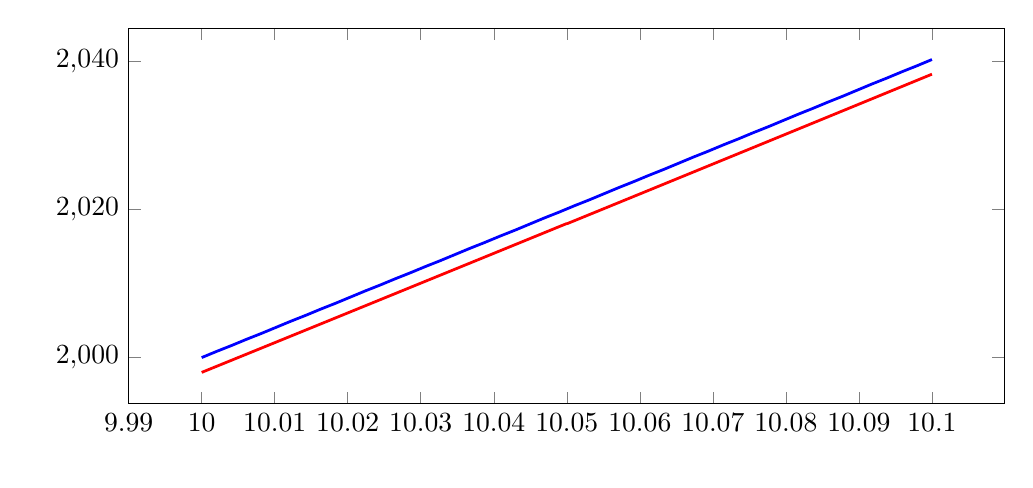
\begin{tikzpicture}[line width=1]
\begin{axis}[width=5in, height=2.5in,
             scatter/classes={a={mark=*,draw=black}},
             xlabel={\mbox{}},
             xlabel style={name=xlabel}, 
             ylabel={\mbox{}}, 
             legend style={
                at={(xlabel.south)},
                yshift=-1ex,
                anchor=north,
                legend cell align=left,
                },
        ]
]
\addplot[draw=red, line width=1] coordinates {(10.0,1998.002)
(10.0001,1998.0421)
(10.0002,1998.0821)
(10.0003,1998.1222)
(10.0004,1998.1622)
(10.0005,1998.2023)
(10.0006,1998.2424)
(10.0007,1998.2824)
(10.0008,1998.3225)
(10.0009,1998.3626)
(10.001,1998.4026)
(10.0011,1998.4427)
(10.0012,1998.4827)
(10.0013,1998.5228)
(10.0014,1998.5629)
(10.0015,1998.6029)
(10.0016,1998.643)
(10.0017,1998.6831)
(10.0018,1998.7231)
(10.0019,1998.7632)
(10.002,1998.8033)
(10.0021,1998.8433)
(10.0022,1998.8834)
(10.0023,1998.9235)
(10.0024,1998.9636)
(10.0025,1999.0036)
(10.0026,1999.0437)
(10.0027,1999.0838)
(10.0028,1999.1238)
(10.0029,1999.1639)
(10.003,1999.204)
(10.0031,1999.244)
(10.0032,1999.2841)
(10.0033,1999.3242)
(10.0034,1999.3643)
(10.0035,1999.4043)
(10.0036,1999.4444)
(10.0037,1999.4845)
(10.0038,1999.5246)
(10.0039,1999.5646)
(10.004,1999.6047)
(10.0041,1999.6448)
(10.0042,1999.6849)
(10.0043,1999.7249)
(10.0044,1999.765)
(10.0045,1999.8051)
(10.0046,1999.8452)
(10.0047,1999.8853)
(10.0048,1999.9253)
(10.0049,1999.9654)
(10.005,2000.0055)
(10.0051,2000.0456)
(10.0052,2000.0857)
(10.0053,2000.1257)
(10.0054,2000.1658)
(10.0055,2000.2059)
(10.0056,2000.246)
(10.0057,2000.2861)
(10.0058,2000.3262)
(10.0059,2000.3662)
(10.006,2000.4063)
(10.0061,2000.4464)
(10.0062,2000.4865)
(10.0063,2000.5266)
(10.0064,2000.5667)
(10.0065,2000.6067)
(10.0066,2000.6468)
(10.0067,2000.6869)
(10.0068,2000.727)
(10.0069,2000.7671)
(10.007,2000.8072)
(10.0071,2000.8473)
(10.0072,2000.8874)
(10.0073,2000.9274)
(10.0074,2000.9675)
(10.0075,2001.0076)
(10.0076,2001.0477)
(10.0077,2001.0878)
(10.0078,2001.1279)
(10.0079,2001.168)
(10.008,2001.2081)
(10.0081,2001.2482)
(10.0082,2001.2883)
(10.0083,2001.3284)
(10.0084,2001.3684)
(10.0085,2001.4085)
(10.0086,2001.4486)
(10.0087,2001.4887)
(10.0088,2001.5288)
(10.0089,2001.5689)
(10.009,2001.609)
(10.0091,2001.6491)
(10.0092,2001.6892)
(10.0093,2001.7293)
(10.0094,2001.7694)
(10.0095,2001.8095)
(10.0096,2001.8496)
(10.0097,2001.8897)
(10.0098,2001.9298)
(10.0099,2001.9699)
(10.01,2002.01)
(10.0101,2002.0501)
(10.0102,2002.0902)
(10.0103,2002.1303)
(10.0104,2002.1704)
(10.0105,2002.2105)
(10.0106,2002.2506)
(10.0107,2002.2907)
(10.0108,2002.3308)
(10.0109,2002.3709)
(10.011,2002.411)
(10.0111,2002.4511)
(10.0112,2002.4912)
(10.0113,2002.5313)
(10.0114,2002.5714)
(10.0115,2002.6115)
(10.0116,2002.6516)
(10.0117,2002.6918)
(10.0118,2002.7319)
(10.0119,2002.772)
(10.012,2002.8121)
(10.0121,2002.8522)
(10.0122,2002.8923)
(10.0123,2002.9324)
(10.0124,2002.9725)
(10.0125,2003.0126)
(10.0126,2003.0527)
(10.0127,2003.0928)
(10.0128,2003.133)
(10.0129,2003.1731)
(10.013,2003.2132)
(10.0131,2003.2533)
(10.0132,2003.2934)
(10.0133,2003.3335)
(10.0134,2003.3736)
(10.0135,2003.4137)
(10.0136,2003.4539)
(10.0137,2003.494)
(10.0138,2003.5341)
(10.0139,2003.5742)
(10.014,2003.6143)
(10.0141,2003.6544)
(10.0142,2003.6946)
(10.0143,2003.7347)
(10.0144,2003.7748)
(10.0145,2003.8149)
(10.0146,2003.855)
(10.0147,2003.8951)
(10.0148,2003.9353)
(10.0149,2003.9754)
(10.015,2004.0155)
(10.0151,2004.0556)
(10.0152,2004.0957)
(10.0153,2004.1359)
(10.0154,2004.176)
(10.0155,2004.2161)
(10.0156,2004.2562)
(10.0157,2004.2963)
(10.0158,2004.3365)
(10.0159,2004.3766)
(10.016,2004.4167)
(10.0161,2004.4568)
(10.0162,2004.497)
(10.0163,2004.5371)
(10.0164,2004.5772)
(10.0165,2004.6173)
(10.0166,2004.6575)
(10.0167,2004.6976)
(10.0168,2004.7377)
(10.0169,2004.7779)
(10.017,2004.818)
(10.0171,2004.8581)
(10.0172,2004.8982)
(10.0173,2004.9384)
(10.0174,2004.9785)
(10.0175,2005.0186)
(10.0176,2005.0588)
(10.0177,2005.0989)
(10.0178,2005.139)
(10.0179,2005.1791)
(10.018,2005.2193)
(10.0181,2005.2594)
(10.0182,2005.2995)
(10.0183,2005.3397)
(10.0184,2005.3798)
(10.0185,2005.4199)
(10.0186,2005.4601)
(10.0187,2005.5002)
(10.0188,2005.5404)
(10.0189,2005.5805)
(10.019,2005.6206)
(10.0191,2005.6608)
(10.0192,2005.7009)
(10.0193,2005.741)
(10.0194,2005.7812)
(10.0195,2005.8213)
(10.0196,2005.8614)
(10.0197,2005.9016)
(10.0198,2005.9417)
(10.0199,2005.9819)
(10.02,2006.022)
(10.0201,2006.0621)
(10.0202,2006.1023)
(10.0203,2006.1424)
(10.0204,2006.1826)
(10.0205,2006.2227)
(10.0206,2006.2628)
(10.0207,2006.303)
(10.0208,2006.3431)
(10.0209,2006.3833)
(10.021,2006.4234)
(10.0211,2006.4636)
(10.0212,2006.5037)
(10.0213,2006.5439)
(10.0214,2006.584)
(10.0215,2006.6241)
(10.0216,2006.6643)
(10.0217,2006.7044)
(10.0218,2006.7446)
(10.0219,2006.7847)
(10.022,2006.8249)
(10.0221,2006.865)
(10.0222,2006.9052)
(10.0223,2006.9453)
(10.0224,2006.9855)
(10.0225,2007.0256)
(10.0226,2007.0658)
(10.0227,2007.1059)
(10.0228,2007.1461)
(10.0229,2007.1862)
(10.023,2007.2264)
(10.0231,2007.2665)
(10.0232,2007.3067)
(10.0233,2007.3468)
(10.0234,2007.387)
(10.0235,2007.4271)
(10.0236,2007.4673)
(10.0237,2007.5075)
(10.0238,2007.5476)
(10.0239,2007.5878)
(10.024,2007.6279)
(10.0241,2007.6681)
(10.0242,2007.7082)
(10.0243,2007.7484)
(10.0244,2007.7886)
(10.0245,2007.8287)
(10.0246,2007.8689)
(10.0247,2007.909)
(10.0248,2007.9492)
(10.0249,2007.9893)
(10.025,2008.0295)
(10.0251,2008.0697)
(10.0252,2008.1098)
(10.0253,2008.15)
(10.0254,2008.1901)
(10.0255,2008.2303)
(10.0256,2008.2705)
(10.0257,2008.3106)
(10.0258,2008.3508)
(10.0259,2008.391)
(10.026,2008.4311)
(10.0261,2008.4713)
(10.0262,2008.5115)
(10.0263,2008.5516)
(10.0264,2008.5918)
(10.0265,2008.632)
(10.0266,2008.6721)
(10.0267,2008.7123)
(10.0268,2008.7525)
(10.0269,2008.7926)
(10.027,2008.8328)
(10.0271,2008.873)
(10.0272,2008.9131)
(10.0273,2008.9533)
(10.0274,2008.9935)
(10.0275,2009.0336)
(10.0276,2009.0738)
(10.0277,2009.114)
(10.0278,2009.1541)
(10.0279,2009.1943)
(10.028,2009.2345)
(10.0281,2009.2747)
(10.0282,2009.3148)
(10.0283,2009.355)
(10.0284,2009.3952)
(10.0285,2009.4354)
(10.0286,2009.4755)
(10.0287,2009.5157)
(10.0288,2009.5559)
(10.0289,2009.5961)
(10.029,2009.6362)
(10.0291,2009.6764)
(10.0292,2009.7166)
(10.0293,2009.7568)
(10.0294,2009.7969)
(10.0295,2009.8371)
(10.0296,2009.8773)
(10.0297,2009.9175)
(10.0298,2009.9577)
(10.0299,2009.9978)
(10.03,2010.038)
(10.0301,2010.0782)
(10.0302,2010.1184)
(10.0303,2010.1586)
(10.0304,2010.1987)
(10.0305,2010.2389)
(10.0306,2010.2791)
(10.0307,2010.3193)
(10.0308,2010.3595)
(10.0309,2010.3996)
(10.031,2010.4398)
(10.0311,2010.48)
(10.0312,2010.5202)
(10.0313,2010.5604)
(10.0314,2010.6006)
(10.0315,2010.6408)
(10.0316,2010.6809)
(10.0317,2010.7211)
(10.0318,2010.7613)
(10.0319,2010.8015)
(10.032,2010.8417)
(10.0321,2010.8819)
(10.0322,2010.9221)
(10.0323,2010.9623)
(10.0324,2011.0024)
(10.0325,2011.0426)
(10.0326,2011.0828)
(10.0327,2011.123)
(10.0328,2011.1632)
(10.0329,2011.2034)
(10.033,2011.2436)
(10.0331,2011.2838)
(10.0332,2011.324)
(10.0333,2011.3642)
(10.0334,2011.4044)
(10.0335,2011.4446)
(10.0336,2011.4848)
(10.0337,2011.5249)
(10.0338,2011.5651)
(10.0339,2011.6053)
(10.034,2011.6455)
(10.0341,2011.6857)
(10.0342,2011.7259)
(10.0343,2011.7661)
(10.0344,2011.8063)
(10.0345,2011.8465)
(10.0346,2011.8867)
(10.0347,2011.9269)
(10.0348,2011.9671)
(10.0349,2012.0073)
(10.035,2012.0475)
(10.0351,2012.0877)
(10.0352,2012.1279)
(10.0353,2012.1681)
(10.0354,2012.2083)
(10.0355,2012.2485)
(10.0356,2012.2887)
(10.0357,2012.3289)
(10.0358,2012.3691)
(10.0359,2012.4093)
(10.036,2012.4495)
(10.0361,2012.4897)
(10.0362,2012.5299)
(10.0363,2012.5702)
(10.0364,2012.6104)
(10.0365,2012.6506)
(10.0366,2012.6908)
(10.0367,2012.731)
(10.0368,2012.7712)
(10.0369,2012.8114)
(10.037,2012.8516)
(10.0371,2012.8918)
(10.0372,2012.932)
(10.0373,2012.9722)
(10.0374,2013.0124)
(10.0375,2013.0526)
(10.0376,2013.0929)
(10.0377,2013.1331)
(10.0378,2013.1733)
(10.0379,2013.2135)
(10.038,2013.2537)
(10.0381,2013.2939)
(10.0382,2013.3341)
(10.0383,2013.3743)
(10.0384,2013.4146)
(10.0385,2013.4548)
(10.0386,2013.495)
(10.0387,2013.5352)
(10.0388,2013.5754)
(10.0389,2013.6156)
(10.039,2013.6558)
(10.0391,2013.6961)
(10.0392,2013.7363)
(10.0393,2013.7765)
(10.0394,2013.8167)
(10.0395,2013.8569)
(10.0396,2013.8971)
(10.0397,2013.9374)
(10.0398,2013.9776)
(10.0399,2014.0178)
(10.04,2014.058)
(10.0401,2014.0982)
(10.0402,2014.1385)
(10.0403,2014.1787)
(10.0404,2014.2189)
(10.0405,2014.2591)
(10.0406,2014.2994)
(10.0407,2014.3396)
(10.0408,2014.3798)
(10.0409,2014.42)
(10.041,2014.4602)
(10.0411,2014.5005)
(10.0412,2014.5407)
(10.0413,2014.5809)
(10.0414,2014.6211)
(10.0415,2014.6614)
(10.0416,2014.7016)
(10.0417,2014.7418)
(10.0418,2014.782)
(10.0419,2014.8223)
(10.042,2014.8625)
(10.0421,2014.9027)
(10.0422,2014.943)
(10.0423,2014.9832)
(10.0424,2015.0234)
(10.0425,2015.0637)
(10.0426,2015.1039)
(10.0427,2015.1441)
(10.0428,2015.1843)
(10.0429,2015.2246)
(10.043,2015.2648)
(10.0431,2015.305)
(10.0432,2015.3453)
(10.0433,2015.3855)
(10.0434,2015.4257)
(10.0435,2015.466)
(10.0436,2015.5062)
(10.0437,2015.5464)
(10.0438,2015.5867)
(10.0439,2015.6269)
(10.044,2015.6671)
(10.0441,2015.7074)
(10.0442,2015.7476)
(10.0443,2015.7879)
(10.0444,2015.8281)
(10.0445,2015.8683)
(10.0446,2015.9086)
(10.0447,2015.9488)
(10.0448,2015.9891)
(10.0449,2016.0293)
(10.045,2016.0695)
(10.0451,2016.1098)
(10.0452,2016.15)
(10.0453,2016.1903)
(10.0454,2016.2305)
(10.0455,2016.2707)
(10.0456,2016.311)
(10.0457,2016.3512)
(10.0458,2016.3915)
(10.0459,2016.4317)
(10.046,2016.472)
(10.0461,2016.5122)
(10.0462,2016.5524)
(10.0463,2016.5927)
(10.0464,2016.6329)
(10.0465,2016.6732)
(10.0466,2016.7134)
(10.0467,2016.7537)
(10.0468,2016.7939)
(10.0469,2016.8342)
(10.047,2016.8744)
(10.0471,2016.9147)
(10.0472,2016.9549)
(10.0473,2016.9952)
(10.0474,2017.0354)
(10.0475,2017.0757)
(10.0476,2017.1159)
(10.0477,2017.1562)
(10.0478,2017.1964)
(10.0479,2017.2367)
(10.048,2017.2769)
(10.0481,2017.3172)
(10.0482,2017.3574)
(10.0483,2017.3977)
(10.0484,2017.4379)
(10.0485,2017.4782)
(10.0486,2017.5184)
(10.0487,2017.5587)
(10.0488,2017.5989)
(10.0489,2017.6392)
(10.049,2017.6795)
(10.0491,2017.7197)
(10.0492,2017.76)
(10.0493,2017.8002)
(10.0494,2017.8405)
(10.0495,2017.8807)
(10.0496,2017.921)
(10.0497,2017.9613)
(10.0498,2018.0015)
(10.0499,2018.0418)
(10.0501,2018.082)
(10.0502,2018.1223)
(10.0503,2018.1626)
(10.0504,2018.2028)
(10.0505,2018.2431)
(10.0506,2018.2833)
(10.0507,2018.3236)
(10.0508,2018.3639)
(10.0509,2018.4041)
(10.051,2018.4444)
(10.0511,2018.4847)
(10.0512,2018.5249)
(10.0513,2018.5652)
(10.0514,2018.6055)
(10.0515,2018.6457)
(10.0516,2018.686)
(10.0517,2018.7263)
(10.0518,2018.7665)
(10.0519,2018.8068)
(10.052,2018.8471)
(10.0521,2018.8873)
(10.0522,2018.9276)
(10.0523,2018.9679)
(10.0524,2019.0081)
(10.0525,2019.0484)
(10.0526,2019.0887)
(10.0527,2019.1289)
(10.0528,2019.1692)
(10.0529,2019.2095)
(10.053,2019.2498)
(10.0531,2019.29)
(10.0532,2019.3303)
(10.0533,2019.3706)
(10.0534,2019.4108)
(10.0535,2019.4511)
(10.0536,2019.4914)
(10.0537,2019.5317)
(10.0538,2019.5719)
(10.0539,2019.6122)
(10.054,2019.6525)
(10.0541,2019.6928)
(10.0542,2019.733)
(10.0543,2019.7733)
(10.0544,2019.8136)
(10.0545,2019.8539)
(10.0546,2019.8942)
(10.0547,2019.9344)
(10.0548,2019.9747)
(10.0549,2020.015)
(10.055,2020.0553)
(10.0551,2020.0955)
(10.0552,2020.1358)
(10.0553,2020.1761)
(10.0554,2020.2164)
(10.0555,2020.2567)
(10.0556,2020.297)
(10.0557,2020.3372)
(10.0558,2020.3775)
(10.0559,2020.4178)
(10.056,2020.4581)
(10.0561,2020.4984)
(10.0562,2020.5387)
(10.0563,2020.5789)
(10.0564,2020.6192)
(10.0565,2020.6595)
(10.0566,2020.6998)
(10.0567,2020.7401)
(10.0568,2020.7804)
(10.0569,2020.8207)
(10.057,2020.8609)
(10.0571,2020.9012)
(10.0572,2020.9415)
(10.0573,2020.9818)
(10.0574,2021.0221)
(10.0575,2021.0624)
(10.0576,2021.1027)
(10.0577,2021.143)
(10.0578,2021.1833)
(10.0579,2021.2236)
(10.058,2021.2638)
(10.0581,2021.3041)
(10.0582,2021.3444)
(10.0583,2021.3847)
(10.0584,2021.425)
(10.0585,2021.4653)
(10.0586,2021.5056)
(10.0587,2021.5459)
(10.0588,2021.5862)
(10.0589,2021.6265)
(10.059,2021.6668)
(10.0591,2021.7071)
(10.0592,2021.7474)
(10.0593,2021.7877)
(10.0594,2021.828)
(10.0595,2021.8683)
(10.0596,2021.9086)
(10.0597,2021.9489)
(10.0598,2021.9892)
(10.0599,2022.0295)
(10.06,2022.0698)
(10.0601,2022.1101)
(10.0602,2022.1504)
(10.0603,2022.1907)
(10.0604,2022.231)
(10.0605,2022.2713)
(10.0606,2022.3116)
(10.0607,2022.3519)
(10.0608,2022.3922)
(10.0609,2022.4325)
(10.061,2022.4728)
(10.0611,2022.5131)
(10.0612,2022.5534)
(10.0613,2022.5937)
(10.0614,2022.634)
(10.0615,2022.6743)
(10.0616,2022.7146)
(10.0617,2022.7549)
(10.0618,2022.7952)
(10.0619,2022.8355)
(10.062,2022.8758)
(10.0621,2022.9161)
(10.0622,2022.9565)
(10.0623,2022.9968)
(10.0624,2023.0371)
(10.0625,2023.0774)
(10.0626,2023.1177)
(10.0627,2023.158)
(10.0628,2023.1983)
(10.0629,2023.2386)
(10.063,2023.2789)
(10.0631,2023.3192)
(10.0632,2023.3596)
(10.0633,2023.3999)
(10.0634,2023.4402)
(10.0635,2023.4805)
(10.0636,2023.5208)
(10.0637,2023.5611)
(10.0638,2023.6014)
(10.0639,2023.6418)
(10.064,2023.6821)
(10.0641,2023.7224)
(10.0642,2023.7627)
(10.0643,2023.803)
(10.0644,2023.8433)
(10.0645,2023.8837)
(10.0646,2023.924)
(10.0647,2023.9643)
(10.0648,2024.0046)
(10.0649,2024.0449)
(10.065,2024.0853)
(10.0651,2024.1256)
(10.0652,2024.1659)
(10.0653,2024.2062)
(10.0654,2024.2465)
(10.0655,2024.2869)
(10.0656,2024.3272)
(10.0657,2024.3675)
(10.0658,2024.4078)
(10.0659,2024.4481)
(10.066,2024.4885)
(10.0661,2024.5288)
(10.0662,2024.5691)
(10.0663,2024.6094)
(10.0664,2024.6498)
(10.0665,2024.6901)
(10.0666,2024.7304)
(10.0667,2024.7707)
(10.0668,2024.8111)
(10.0669,2024.8514)
(10.067,2024.8917)
(10.0671,2024.9321)
(10.0672,2024.9724)
(10.0673,2025.0127)
(10.0674,2025.053)
(10.0675,2025.0934)
(10.0676,2025.1337)
(10.0677,2025.174)
(10.0678,2025.2144)
(10.0679,2025.2547)
(10.068,2025.295)
(10.0681,2025.3354)
(10.0682,2025.3757)
(10.0683,2025.416)
(10.0684,2025.4564)
(10.0685,2025.4967)
(10.0686,2025.537)
(10.0687,2025.5774)
(10.0688,2025.6177)
(10.0689,2025.658)
(10.069,2025.6984)
(10.0691,2025.7387)
(10.0692,2025.779)
(10.0693,2025.8194)
(10.0694,2025.8597)
(10.0695,2025.9)
(10.0696,2025.9404)
(10.0697,2025.9807)
(10.0698,2026.0211)
(10.0699,2026.0614)
(10.07,2026.1017)
(10.0701,2026.1421)
(10.0702,2026.1824)
(10.0703,2026.2228)
(10.0704,2026.2631)
(10.0705,2026.3034)
(10.0706,2026.3438)
(10.0707,2026.3841)
(10.0708,2026.4245)
(10.0709,2026.4648)
(10.071,2026.5052)
(10.0711,2026.5455)
(10.0712,2026.5859)
(10.0713,2026.6262)
(10.0714,2026.6665)
(10.0715,2026.7069)
(10.0716,2026.7472)
(10.0717,2026.7876)
(10.0718,2026.8279)
(10.0719,2026.8683)
(10.072,2026.9086)
(10.0721,2026.949)
(10.0722,2026.9893)
(10.0723,2027.0297)
(10.0724,2027.07)
(10.0725,2027.1104)
(10.0726,2027.1507)
(10.0727,2027.1911)
(10.0728,2027.2314)
(10.0729,2027.2718)
(10.073,2027.3121)
(10.0731,2027.3525)
(10.0732,2027.3928)
(10.0733,2027.4332)
(10.0734,2027.4735)
(10.0735,2027.5139)
(10.0736,2027.5542)
(10.0737,2027.5946)
(10.0738,2027.6349)
(10.0739,2027.6753)
(10.074,2027.7157)
(10.0741,2027.756)
(10.0742,2027.7964)
(10.0743,2027.8367)
(10.0744,2027.8771)
(10.0745,2027.9174)
(10.0746,2027.9578)
(10.0747,2027.9982)
(10.0748,2028.0385)
(10.0749,2028.0789)
(10.075,2028.1192)
(10.0751,2028.1596)
(10.0752,2028.2)
(10.0753,2028.2403)
(10.0754,2028.2807)
(10.0755,2028.321)
(10.0756,2028.3614)
(10.0757,2028.4018)
(10.0758,2028.4421)
(10.0759,2028.4825)
(10.076,2028.5229)
(10.0761,2028.5632)
(10.0762,2028.6036)
(10.0763,2028.6439)
(10.0764,2028.6843)
(10.0765,2028.7247)
(10.0766,2028.765)
(10.0767,2028.8054)
(10.0768,2028.8458)
(10.0769,2028.8861)
(10.077,2028.9265)
(10.0771,2028.9669)
(10.0772,2029.0073)
(10.0773,2029.0476)
(10.0774,2029.088)
(10.0775,2029.1284)
(10.0776,2029.1687)
(10.0777,2029.2091)
(10.0778,2029.2495)
(10.0779,2029.2898)
(10.078,2029.3302)
(10.0781,2029.3706)
(10.0782,2029.411)
(10.0783,2029.4513)
(10.0784,2029.4917)
(10.0785,2029.5321)
(10.0786,2029.5725)
(10.0787,2029.6128)
(10.0788,2029.6532)
(10.0789,2029.6936)
(10.079,2029.734)
(10.0791,2029.7743)
(10.0792,2029.8147)
(10.0793,2029.8551)
(10.0794,2029.8955)
(10.0795,2029.9358)
(10.0796,2029.9762)
(10.0797,2030.0166)
(10.0798,2030.057)
(10.0799,2030.0974)
(10.08,2030.1377)
(10.0801,2030.1781)
(10.0802,2030.2185)
(10.0803,2030.2589)
(10.0804,2030.2993)
(10.0805,2030.3396)
(10.0806,2030.38)
(10.0807,2030.4204)
(10.0808,2030.4608)
(10.0809,2030.5012)
(10.081,2030.5416)
(10.0811,2030.5819)
(10.0812,2030.6223)
(10.0813,2030.6627)
(10.0814,2030.7031)
(10.0815,2030.7435)
(10.0816,2030.7839)
(10.0817,2030.8242)
(10.0818,2030.8646)
(10.0819,2030.905)
(10.082,2030.9454)
(10.0821,2030.9858)
(10.0822,2031.0262)
(10.0823,2031.0666)
(10.0824,2031.107)
(10.0825,2031.1474)
(10.0826,2031.1877)
(10.0827,2031.2281)
(10.0828,2031.2685)
(10.0829,2031.3089)
(10.083,2031.3493)
(10.0831,2031.3897)
(10.0832,2031.4301)
(10.0833,2031.4705)
(10.0834,2031.5109)
(10.0835,2031.5513)
(10.0836,2031.5917)
(10.0837,2031.6321)
(10.0838,2031.6725)
(10.0839,2031.7129)
(10.084,2031.7532)
(10.0841,2031.7936)
(10.0842,2031.834)
(10.0843,2031.8744)
(10.0844,2031.9148)
(10.0845,2031.9552)
(10.0846,2031.9956)
(10.0847,2032.036)
(10.0848,2032.0764)
(10.0849,2032.1168)
(10.085,2032.1572)
(10.0851,2032.1976)
(10.0852,2032.238)
(10.0853,2032.2784)
(10.0854,2032.3188)
(10.0855,2032.3592)
(10.0856,2032.3996)
(10.0857,2032.44)
(10.0858,2032.4804)
(10.0859,2032.5208)
(10.086,2032.5612)
(10.0861,2032.6017)
(10.0862,2032.6421)
(10.0863,2032.6825)
(10.0864,2032.7229)
(10.0865,2032.7633)
(10.0866,2032.8037)
(10.0867,2032.8441)
(10.0868,2032.8845)
(10.0869,2032.9249)
(10.087,2032.9653)
(10.0871,2033.0057)
(10.0872,2033.0461)
(10.0873,2033.0865)
(10.0874,2033.1269)
(10.0875,2033.1674)
(10.0876,2033.2078)
(10.0877,2033.2482)
(10.0878,2033.2886)
(10.0879,2033.329)
(10.088,2033.3694)
(10.0881,2033.4098)
(10.0882,2033.4502)
(10.0883,2033.4906)
(10.0884,2033.5311)
(10.0885,2033.5715)
(10.0886,2033.6119)
(10.0887,2033.6523)
(10.0888,2033.6927)
(10.0889,2033.7331)
(10.089,2033.7735)
(10.0891,2033.814)
(10.0892,2033.8544)
(10.0893,2033.8948)
(10.0894,2033.9352)
(10.0895,2033.9756)
(10.0896,2034.016)
(10.0897,2034.0565)
(10.0898,2034.0969)
(10.0899,2034.1373)
(10.09,2034.1777)
(10.0901,2034.2181)
(10.0902,2034.2586)
(10.0903,2034.299)
(10.0904,2034.3394)
(10.0905,2034.3798)
(10.0906,2034.4203)
(10.0907,2034.4607)
(10.0908,2034.5011)
(10.0909,2034.5415)
(10.091,2034.5819)
(10.0911,2034.6224)
(10.0912,2034.6628)
(10.0913,2034.7032)
(10.0914,2034.7436)
(10.0915,2034.7841)
(10.0916,2034.8245)
(10.0917,2034.8649)
(10.0918,2034.9053)
(10.0919,2034.9458)
(10.092,2034.9862)
(10.0921,2035.0266)
(10.0922,2035.0671)
(10.0923,2035.1075)
(10.0924,2035.1479)
(10.0925,2035.1883)
(10.0926,2035.2288)
(10.0927,2035.2692)
(10.0928,2035.3096)
(10.0929,2035.3501)
(10.093,2035.3905)
(10.0931,2035.4309)
(10.0932,2035.4714)
(10.0933,2035.5118)
(10.0934,2035.5522)
(10.0935,2035.5927)
(10.0936,2035.6331)
(10.0937,2035.6735)
(10.0938,2035.714)
(10.0939,2035.7544)
(10.094,2035.7948)
(10.0941,2035.8353)
(10.0942,2035.8757)
(10.0943,2035.9162)
(10.0944,2035.9566)
(10.0945,2035.997)
(10.0946,2036.0375)
(10.0947,2036.0779)
(10.0948,2036.1183)
(10.0949,2036.1588)
(10.095,2036.1992)
(10.0951,2036.2397)
(10.0952,2036.2801)
(10.0953,2036.3205)
(10.0954,2036.361)
(10.0955,2036.4014)
(10.0956,2036.4419)
(10.0957,2036.4823)
(10.0958,2036.5228)
(10.0959,2036.5632)
(10.096,2036.6036)
(10.0961,2036.6441)
(10.0962,2036.6845)
(10.0963,2036.725)
(10.0964,2036.7654)
(10.0965,2036.8059)
(10.0966,2036.8463)
(10.0967,2036.8868)
(10.0968,2036.9272)
(10.0969,2036.9677)
(10.097,2037.0081)
(10.0971,2037.0486)
(10.0972,2037.089)
(10.0973,2037.1294)
(10.0974,2037.1699)
(10.0975,2037.2103)
(10.0976,2037.2508)
(10.0977,2037.2912)
(10.0978,2037.3317)
(10.0979,2037.3722)
(10.098,2037.4126)
(10.0981,2037.4531)
(10.0982,2037.4935)
(10.0983,2037.534)
(10.0984,2037.5744)
(10.0985,2037.6149)
(10.0986,2037.6553)
(10.0987,2037.6958)
(10.0988,2037.7362)
(10.0989,2037.7767)
(10.099,2037.8171)
(10.0991,2037.8576)
(10.0992,2037.8981)
(10.0993,2037.9385)
(10.0994,2037.979)
(10.0995,2038.0194)
(10.0996,2038.0599)
(10.0997,2038.1003)
(10.0998,2038.1408)
(10.0999,2038.1813)
(10.1,2038.2217)};\node[pin=below right:{$y=|20 \frac{n^5}{n^3 + 1}|$}] at (axis cs:10.5,2203.0968820800517) {};\addplot[draw=blue, line width=1] coordinates {(10.0,2000.0)
(10.002,2000.8164)
(10.0041,2001.633)
(10.0061,2002.4497)
(10.0082,2003.2666)
(10.0102,2004.0837)
(10.0122,2004.901)
(10.0143,2005.7184)
(10.0163,2006.5359)
(10.0184,2007.3537)
(10.0204,2008.1716)
(10.0224,2008.9897)
(10.0245,2009.8079)
(10.0265,2010.6263)
(10.0286,2011.4449)
(10.0306,2012.2636)
(10.0327,2013.0825)
(10.0347,2013.9016)
(10.0367,2014.7209)
(10.0388,2015.5403)
(10.0408,2016.3599)
(10.0429,2017.1796)
(10.0449,2017.9995)
(10.0469,2018.8196)
(10.049,2019.6398)
(10.051,2020.4602)
(10.0531,2021.2808)
(10.0551,2022.1015)
(10.0571,2022.9224)
(10.0592,2023.7435)
(10.0612,2024.5648)
(10.0633,2025.3862)
(10.0653,2026.2077)
(10.0673,2027.0295)
(10.0694,2027.8514)
(10.0714,2028.6735)
(10.0735,2029.4957)
(10.0755,2030.3181)
(10.0776,2031.1407)
(10.0796,2031.9634)
(10.0816,2032.7863)
(10.0837,2033.6094)
(10.0857,2034.4327)
(10.0878,2035.2561)
(10.0898,2036.0796)
(10.0918,2036.9034)
(10.0939,2037.7273)
(10.0959,2038.5514)
(10.098,2039.3756)
(10.1,2040.2)};\node[pin=above left:{$y=20n^2$}] at (axis cs:10.5,2205.0) {};
\end{axis}\end{tikzpicture}\end{center}

If we choose $C = 4$ and $N = 37$,
we see that for $n \geq N$,
\[
\left|
-3n^{3.5} + 42 \frac{n^5}{n^2 + 1}
\right| 
\leq C
\left|
n^4
\right|
\]
i.e.,
\[
|f(n)| \leq C|g(n)|
\]
Hence
\[
f(n) = O(n^4)
\]
\qed
